\chapter{Separación}%
\label{cha:separacion}
En este apartado vamos a estudiar la noción de separación en profundidad. Veremos que propiedades tienen los espacios que poseen esta característica y qué consecuencias tiene tenerla sobre el resto de la topología del mismo.

\section{Definición y propiedades}%
\label{sec:concepto}

En primer lugar, vamos a tratar de definir el concepto de separación. Al principio, es un poco complicado asumir que esta propiedad no tiene que cumplirse trivialmente porque estamos muy mal acostumbrados con $\mathbb{R}^n$, pero es importante distinguir aquellos espacios donde no podemos separar claramente dos puntos.

\begin{defi}[Espacio Hausdoff o $T_2$]
Sea $X$ un espacio topológico, decimos que es \textbf{Hausdorff o $T_2$} si y sólo si para todo par de puntos distintos $x, y \in X$ existen algunos entornos de cada uno disjuntos entre sí.
\end{defi}

\begin{prop}
Sea $X$ un espacio topológico, si es Hausdorff podemos encontrar dichos entornos abiertos y disjuntos.
\end{prop}
\begin{demo}
Para cada entorno $V \ent X$, por ser entorno, existe $U\ab X$ y $U\subset V$ que también es entorno. Escogiendo a esos dos abiertos (uno en cada entorno) siguen siendo disjuntos y cumplen la definición de $T_2$.
\end{demo}

\begin{prop}
Sea $X$ un espacio topológico Hausdorff, entonces los puntos son cerrados.
\end{prop}
\begin{demo}    
Para cualquier $x \in X$ y cualquier $y \in X \setminus \left\{ x \right\}$, por ser Hausdorff, existe un entorno abierto $U^y \not\ni x$. Por tanto, podemos escribir el complementario de $\{x\}$ como la unión de todos esos entornos para los puntos que no son $x$, es decir, $X \setminus \{x\} = \bigcup_{y \neq x} U^y$ y como el complementario es unión de abiertos, $\{x\}$ es cerrado.
\end{demo}

\begin{obs}
\begin{enumerate}
    \item Un espacio topológico con la topología de los complementarios finitos $\left( X, \mathcal{T}_{\text{CF}} \right)$ no es Hausdorff y, sin embargo, tiene puntos cerrados.
    
    No es Hausdorff porque, si $X$ es infinito, dos abiertos cualesquiera se cortan ya que si cogemos dos abiertos $U_1, U_2 \in \mathcal{T}_{\text{CF}}$, como sus complementarios $X \setminus U_1$ y $X \setminus U_2$ son finitos y $X$ es infinito, entonces siempre podremos encontrar un $x \not\in X \setminus U_1 \cup X \setminus U_2$, es decir, que $x \in U_1 \cap U_2$. 

    \item Si una topología contiene a una topología Hausdorff, entonces también es Hausdorff.
    
    Este es precisamente el caso de la radial $\mathcal{T}_{\text{rad}}$ que contiene a la usual $\mathcal{T}_{u}$, que es Hausdorff.
	Que la usual es Hausdorff es sencillo, pues para dos puntos $x$ e $y$ distintos basta con escoger $B\left( x, \varepsilon \right)$ y $B\left( y, \varepsilon \right)$ que son disjuntos si tomamos $\varepsilon < \frac{\lVert x - y \rVert}{2}$. Ahora ver que la radial es Hausdorff es trivial, pues como los abiertos usuales son abiertos radiales podemos coger las mismas bolas como entornos.

    \item En la topología del punto $\left( X, \mathcal{T}_a \right)$ el punto clave $a$ no es cerrado, lo que impide que sea Hausdorff. 
    
    Si el punto $a$ fuera cerrado, el conjunto $X\setminus\{a\}$ sería abierto, pero en esta topología la definición de abierto es contener al punto $a$ y precisamente $X\setminus\{a\}$ no lo contiene por definición.
\end{enumerate}
\end{obs}

A continuación, lo que vamos a ver es uno de los teoremas más habituales y útiles que hemos venido utilizando en el Análisis en general. En primer lugar, el conjunto de puntos donde dos funciones coinciden es cerrado (o donde una toma un cierto valor también porque se puede considerar dicho valor como la aplicación constante ese valor) y, en segundo lugar, si dos funciones coinciden en un conjunto denso, entonces coinciden en todos sus puntos.

\begin{prop}
Sean $f, g: X \rightarrow Y$ dos funciones continuas e $Y$ un espacio topológico Hausdorff, entonces el conjunto de puntos donde coinciden:
\[
\{f = g\} = \{x \in X : f\left( x \right) = g\left( x \right)\}
\]
es un conjunto cerrado.
\end{prop}
\begin{demo}
Para demostrar que nuestro conjunto es cerrado habrá que demostrar que el complementario es abierto, es decir, que si un punto cumple $f\left( x \right) \neq g\left( x \right)$ entonces habrá un entorno suyo cuyos puntos también verificarán $f\left( y \right) \neq g\left( y \right)$. Con esto, tendremos que $\left\{ f \neq g \right\}$ es entorno de todos sus puntos y, por tanto, abierto.

Si $f\left( x \right) \neq g\left( x \right)$, entonces por ser $T_2$, $\exists V^{f\left( x \right)} \cap V^{g\left( x \right)} = \emptyset$. Como la aplicación $f$ es continua, entonces $f^{-1}V^{f\left( x \right)}$ y $g^{-1}V^{g\left( x \right)}$ son entornos de $x$ y, por tanto, su intersección $f^{-1}V^{f\left( x \right)} \cap g^{-1}V^{g\left( x \right)} = W^x$ es también entorno de $x$ (y es no vacío porque $x$ pertenece a él).

Si observamos ahora la intersección de $W^x$ con el complementario $\{f=g\}$, entonces vemos que:
\[
\forall y \in V^x \Rightarrow
\begin{cases}
        f\left( y \right) \in V^{f\left( x \right)} \\
        g\left( y \right) \in V^{g\left( x \right)} 
\end{cases}
\stackrel{V^{f(x)}\cap V^{g(x)} = \emptyset}{\Rightarrow} f \left( y \right) \neq g\left( y \right)
\]
es decir, que $W^x\cap \{f=g\} = \emptyset$, luego $W^x\subset \{f\neq g\}$.
\end{demo}

\begin{coro}[Extensión por continuidad a la adherencia]
Sean $f, g: X \rightarrow Y$ dos funciones continuas, $Y$ un espacio topológico Hausdorff y $\left\{ f = g \right\}$ es denso\footnote{Esto quiere decir que existe un subconjunto $A\subset X$ denso donde las funciones coinciden.}, entonces $f \equiv g$.
\end{coro}
\begin{demo}
Si $f$ y $g$ coinciden en un subconjunto $A$, entonces $\{f = g\} \supset A$ y como $\{f = g\}$ es cerrado, entonces $\{f = g\} \supset \overline{A}$. Como $A$ es denso, entonces $\overline{A} = X$ y esto implica que $\{f=g\}\supset X$, es decir, que $\{f=g\} = X$.
\end{demo}

Con este último corolario, reafirmamos lo comentado al inicio. Cuando se dan las condiciones adecuadas en un espacio Hausdorff, podemos extender una función en un conjunto a su adherencia.

\begin{obs}
Tiene especial relevancia que el espacio real usual $\mathbb{R}$ sea Hausdorff y vamos a ver por qué. Si tenemos una función $f: X \rightarrow Y$ continua donde $Y$ es Hausdorff, entonces la preimagen $f^{-1}\left( y \right)$ de cualquier $y\in Y$ es un cerrado de $X$ porque hemos visto que en estas condiciones los puntos de $Y$ son cerrados y la preimagen de cerrados por continuidad es cerrada.

¿Por qué es entonces relevante que $\mathbb{R}$ sea Hausdorff? Porque este último resultado implica que cualquier conjunto del estilo $\{x\in X : f(x) = \alpha \mbox{ donde } \alpha \in \mathbb{R}\}$ es un conjunto cerrado, puesto que dicho conjunto en realidad es $f^{-1}(\alpha)$ y $\alpha$ es cerrado.
\end{obs}

\section{Tabla de comportamiento}%
\label{sec:tabla_de_comportamiento}
En este apartado estudiamos como comporta la propiedad definida con respecto a las construcciones del tema \nameref{cha:construcciones}. Se trata de ver cuándo se conserva, cuándo no y qué hipótesis podemos añadir para que se conserve en los casos que no.

\begin{table}[H]
\centering
\begin{tabular}{| c | c | c | c | c |}
    \hline
    & Subespacios & Cocientes & Productos & Sumas\\
    \hline
    $T_2$ & $\Rightarrow$ & \ding{55} & $\Leftrightarrow$ & $\Leftrightarrow$\\
    \hline
\end{tabular}
\caption{Tabla de comportamiento de la separación.}
\end{table}

\begin{demo}
\begin{enumerate}
    \item \textbf{Subespacios}:
    
    Consideremos un subespacio $Y\subset X$ de un espacio $X$ que es Hausdorff. Por ser $X$ Hausdorff, cualesquiera dos puntos $y_1, y_2 \in Y$ verifican que $\exists V^{y_1} \cap V^{y_2} = \emptyset$ donde $V^{y_1}$ y $V^{y_2}$ son entornos en $X$. Pues si tomamos los correspondientes entornos, pero en la topología relativa a $Y$, entonces $\left( V^{y_1} \cap Y \right) \cap \left( V^{y_2} \cap Y \right) = \emptyset$ vemos que siguen sin cortarse.

    \item \textbf{Cociente}:
    
    Para demostrar que no se cumple basta con dar un contraejemplo: consideremos el cociente y los respectivos puntos
\[
Y = \faktor{\mathbb{R}}{\mathbb{Q}}: \begin{rcases}
        y_1 = \mathbb{Q} \in Y\\
        y_2 = \sqrt{2} \in Y
    \end{rcases}
\]
y veamos que $\nexists V^{y_1} \cap V^{y_2} = \emptyset$. Cualquier entorno abierto de $\sqrt{2}$ contiene racionales (por su densidad en $\mathbb{R}$), por tanto al saturar contiene $\mathbb{Q}$. Como todo abierto en el cociente es proyección de un saturado, cualquier abierto contiene al punto gordo $\mathbb{Q}$ y, en consecuencia, la intersección nunca es disjunta.

    \item \textbf{Producto}
    
    Veamos que se da la doble implicación, es decir, que $X$ e $Y$ son ambos $T_2$ si y sólo si $X \times Y$ es $T_2$.
    \begin{itemize}
        \item[$\Rightarrow)$] Tomamos $\left( x_1, y_1 \right) \neq \left( x_2, y_2 \right) \in X \times Y$. Esto es posible en dos casos:
        \begin{itemize}
            \item $x_1 \neq x_2$. Como $X$ es $T_2 \Rightarrow \exists V^{x_1} \cap V^{x_2} = \emptyset \Rightarrow \left( V^{x_1} \times Y \right) \cap \left( V^{x_2} \times Y \right) = \emptyset$ 
            \item $y_1 \neq y_2$ podemos hacer lo mismo porque $Y$ es también $T_2$.
        \end{itemize}

    %TODO: Corregir caption 
    \begin{figure}[H]
        \centering
        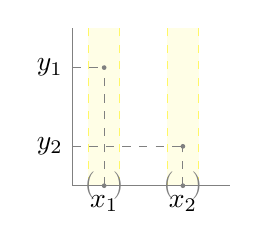
\begin{tikzpicture}
            \draw[-, gray] (0,0) -- (0,2);

            %Rectangulo izq
            \fill[fill=yellow!10, very thick, dashed] (0.2,2) rectangle (0.6,0);
            \draw[-, yellow!60] (0.2,0) -- (0.6,0);
            \draw[-, yellow!60, dashed] (0.2,0) -- (0.2,2);
            \draw[-, yellow!60, dashed] (0.6,0) -- (0.6,2);
            \fill[gray] (0.4,0) circle (0.03);

            %Rectangulo der
            \fill[fill=yellow!10, very thick, dashed] (1.2,2) rectangle (1.6,0);
            \draw[-, yellow!60] (1.2,0) -- (1.6,0);
            \draw[-, yellow!60, dashed] (1.2,0) -- (1.2,2);
            \draw[-, yellow!60, dashed] (1.6,0) -- (1.6,2);
            \fill[gray] (1.4,0) circle (0.03);

            \draw[-, gray] (0,0) -- (2,0) node[pos=0.11] {(}
                node[pos=0.29] {)}
                node[pos=0.61] {(}
                node[pos=0.79] {)};
            postaction={decorate}

            \node(x1) at (0.4,0) [below] {$x_1$};
            \node(x2) at (1.4,0) [below] {$x_2$};

            \fill[gray] (0.4,1.5) circle (0.03);
            \fill[gray] (1.4,0.5) circle (0.03);

            \node(y1) at (0,1.5) [left] {$y_1$};
            \node(y2) at (0,0.5) [left] {$y_2$};

            %Lineas 1
            \draw[-, gray, dashed] (x1) -- (0.4,1.5);
            \draw[-, gray, dashed] (y1) -- (0.4,1.5);

            %Lineas 2
            \draw[-, gray, dashed] (x2) -- (1.4,0.5);
            \draw[-, gray, dashed] (y2) -- (1.4,0.5);
        \end{tikzpicture}
        \captionsetup{font={color=gray}}
        \caption{Separación en el producto gracias a la separación en el factor.}
    \end{figure}

    \item[$\Leftarrow)$] Sabemos que $X \approx X \times \left\{ y_0 \right\} \subset X \times Y$. Como $X\times Y$ es $T_2$ y hemos visto que esta propiedad se hereda por subespacios, entonces $X_0\times \left\{ y_0 \right\}$ es $T_2$ y, por homeomorfismo, $X$ también.
    \end{itemize} 

    \item \textbf{Suma}:
    
    Recordemos que se ha definido la suma como la unión disjunta de los sumandos. Esto quiere decir que para cualquier $x\in X$ el propio $X$ es entorno de $x$ y lo mismo ocurre con $Y$ para sus puntos. Esto quiere decir que $X=V^x$, $Y=V^y$ y $V^x \cap V^y = X\cap Y = \emptyset$. Por tanto, los puntos de distintos conjuntos lo verifican.
    
    Si $X$ y $Y$ son ambos $T_2$, entonces la suma lo es porque hemos visto que entre conjuntos se cumple y si son $T_2$ dentro del propio conjunto se cumple también. Pero es que además el recíproco es cierto, pues si se cumple en la suma se debe cumplir en cada uno de los conjuntos.
\end{enumerate}    
\end{demo}
